\textbf{Beispiel 2}\\ \\
a)\\ \\
\begin{figure}[h]
	\centering
	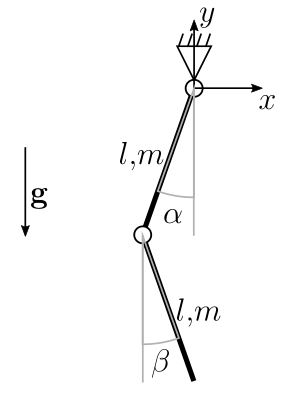
\includegraphics[width= 3cm]{tikz/02_02_2018_2a}
\end{figure}
\newline 
Dieses Doppelpendel besitzt zwei Freiheitsgrade. Die geeignete Wahl für die generalisierten Koordinaten lautet
\[
	\textbf{q} = \begin{bmatrix}
		\alpha \\
		\beta 
	\end{bmatrix}
\]
b) \\ \\
Die beiden Ortsvektoren zu den Schwerpunkten der Pendelstäbe lauten
\begin{align*}
	\textbf{a} = \frac{l}{2} \begin{bmatrix}
		\sin(\alpha) \\
		-\cos(\alpha)
	\end{bmatrix}
	\\
	\textbf{b} = \frac{l}{2}\begin{bmatrix}
		\sin(\beta) \\
		-\cos(\beta)
	\end{bmatrix}
	+ l \begin{bmatrix}
		\sin(\alpha) \\
		-\cos(\alpha)
	\end{bmatrix}
\end{align*}
c)\\ \\
Die Formel für das Massenträgheitsmoment kann aus der Formelsammlung entnommen werden. Dieses lautet daher
\[	
	\varTheta = \int_{-\frac{l}{2}}^{\frac{l}{2}}r^2\text{d}m = \frac{m}{l}\int_{-\frac{l}{2}}^{\frac{l}{2}}r^2\text{d}r = \frac{ml^2}{12}
\]
Die notwendigen Zeitableitungen, die später für die kinetische Energie benötigt werden lauten 
\begin{align*}
	\dot{\textbf{a}} &= \frac{l\dot{\alpha}}{2}\begin{bmatrix}
		\cos(\alpha) \\
		\sin(\alpha)
	\end{bmatrix}
	\\
	\dot{\textbf{b}} &= \frac{l\dot{\beta}}{2}\begin{bmatrix}
		\cos(\beta) \\
		\sin(\beta)
	\end{bmatrix}
	+ l\dot{\alpha}\begin{bmatrix}
		\cos(\alpha) \\
		\sin(\alpha)
	\end{bmatrix}
\end{align*}
Die Betragsquadrate dieser Vektoren lauten
\begin{align*}
	||\dot{\textbf{a}}||_2^2 &= \frac{l^2\dot{\alpha}^2}{4} \\
	||\dot{\textbf{b}}||_2^2 &= \left(\frac{l\dot{\beta}}{2}\cos(\beta) + l\dot{\alpha}\cos(\alpha)\right)^2 + \left(\frac{l\dot{\beta}}{2}\sin(\beta) + l\dot{\alpha}\sin(\alpha)\right)^2 \\
	&= \frac{l^2\dot{\beta}^2}{4}\cos^2(\beta) + l^2\dot{\beta}\dot{\alpha}\cos(\alpha)\cos(\beta) + l^2\dot{\alpha}^2\cos^2(\alpha) + \frac{l^2\dot{\beta}^2}{4}\sin^2(\beta) + l^2\dot{\beta}\dot{\alpha}\sin(\alpha)\sin(\beta) + l^2\dot{\alpha}^2\sin^2(\alpha) \\
	&= \frac{l^2\dot{\beta}^2}{4} + l^2\dot{\alpha}^2 + l^2\dot{\alpha}\dot{\beta}\cos(\alpha - \beta)
\end{align*}
Somit lautet die kinetische Energie
\begin{align*}
	T &= \frac{1}{2}m\left(\frac{l^2\dot{\alpha}^2}{4} + \frac{l^2\dot{\beta}^2}{4} + l^2\dot{\alpha}^2 + l^2\dot{\alpha}\dot{\beta}\cos(\alpha - \beta)\right) \\
	&= ml^2\left(\frac{2}{3}\dot{\alpha}^2 + \frac{1}{6}\dot{\beta} + \frac{1}{2}l^2\cos(\alpha - \beta)\dot{\alpha}\dot{\beta}\right)	
\end{align*}
e)\\ \\
Die potentielle Energie des Gesamtsystems lautet
\begin{align*}
	V &= -mg\frac{l}{2}\cos(\alpha) - mg\left(\frac{l}{2}\cos(\beta) + l\cos(\alpha)\right) \\
	  &= -\left(\frac{3}{2}\cos(\alpha) + \frac{1}{2}\cos(\beta)\right)
\end{align*}
e)\\ \\
Mit der Lagrange-Funktion und der Formel für den Euler-Lagrange-Formalismus folgt
\[
	\frac{\text{d}}{\text{d}t}\frac{\partial}{\partial \dot{\textbf{q}}}T = -\frac{\partial}{\partial \textbf{q}}V + \textbf{f}_e^T\left(\frac{\partial \textbf{a}}{\partial \textbf{q}} + \frac{\partial \textbf{b}}{\partial \textbf{q}}\right)
\]
Betrachtet man nun den Fall $V = 0$ muss die Erdbeschleunigung als externe Kraft angesetzt werden.
\[
	\textbf{f}_e = \begin{bmatrix}
		0  \\
		-mg
	\end{bmatrix}
\]
\newpage
\noindent
Nun müssen die gezeigt das die beiden Bedingungen aus den Euler-Lagrange-Formalismus
\[
	-\frac{\partial V}{\partial \alpha} = \textbf{f}_e^T\left(\frac{\partial \textbf{a}}{\partial \textbf{q}} + \frac{\partial \textbf{b}}{\partial \textbf{q}}\right) \quad \text{und} \quad -\frac{\partial V}{\partial \beta} = \textbf{f}_e^T\left(\frac{\partial \textbf{a}}{\partial \textbf{q}} + \frac{\partial \textbf{b}}{\partial \textbf{q}}\right) = \textbf{f}_e^T\frac{\partial \textbf{b}}{\partial \beta}
\]
Durch die Ermittlung dieser vier Terme sieht man
\begin{align*}
		-\frac{\partial V}{\partial \alpha} &= -\frac{3mgl}{2}\sin(\alpha) \\
		\textbf{f}_e^T\left(\frac{\partial \textbf{a}}{\partial \textbf{q}} + \frac{\partial \textbf{b}}{\partial \textbf{q}}\right) &= -mg\frac{3l}{2}\sin(\alpha)
\end{align*}
und
\begin{align*}
	-\frac{\partial V}{\partial \beta} &= -\frac{mgl}{2}\sin(\beta) \\
	\textbf{f}_e^T\frac{\partial \textbf{b}}{\partial \beta} &= -mg\frac{l}{2}
\end{align*}